% =============================================================
%  Urban Waste Detection — vertical poster (A0 portrait, EN)
%  Compile: pdflatex poster.tex
% =============================================================
\documentclass[25pt, a0paper, portrait, margin=12mm, innermargin=12mm,
               blockverticalspace=6mm, colspace=10mm]{tikzposter}

\usepackage[utf8]{inputenc}
\usepackage[T1]{fontenc}
\usepackage{graphicx}
\usepackage{booktabs}
\usepackage{multirow}
\usepackage{amsmath}
\graphicspath{{../figuras_final/}{../figuras_p0/}}

% ── project palette ──────────────────────────────────────────
\definecolor{inkA}{HTML}{1A1A19}
\definecolor{inkB}{HTML}{52514E}
\definecolor{surface}{HTML}{FCFCFB}
\definecolor{acBlue}{HTML}{2A78D6}
\definecolor{acOrange}{HTML}{EB6834}
\definecolor{acGreen}{HTML}{1BAF7A}
\definecolor{acRed}{HTML}{C0392B}

\usetheme{Simple}
\colorlet{backgroundcolor}{surface}
\colorlet{framecolor}{surface}
\colorlet{titlebgcolor}{inkA}
\colorlet{titlefgcolor}{surface}
\colorlet{blocktitlefgcolor}{inkA}
\colorlet{blockbodyfgcolor}{inkA}
\tikzposterlatexaffectionproofoff

\newcommand{\keynum}[2]{%
  \begin{minipage}{0.23\linewidth}\centering
  {\fontsize{50}{52}\selectfont\bfseries\color{acOrange}#1}\\[2mm]
  {\large\color{inkB}#2}
  \end{minipage}}

\title{\parbox{0.94\linewidth}{\centering \raisebox{-0.12ex}{\rotatebox[origin=c]{180}{?}}Qu\'e tan lejos viaja un detector de basura?\\[2mm]
 {\fontsize{28}{33}\selectfont Detecci\'on cross-domain de residuos urbanos en
 im\'agenes de mano, dashcam y dron}}}
\author{Jairzinho Santos}
\institute{Universidad Nacional de Ingenier\'ia, Lima, Per\'u \quad---\quad
 Visi\'on Computacional, Maestr\'ia en Inteligencia Artificial, 2026-I \quad---\quad
 Prof.\ Elian Laura Riveros}

\begin{document}
\maketitle

% ═════════════════════ ROW 1 ═════════════════════
\begin{columns}
\column{0.5}
\block{La pregunta}{
Los benchmarks de detecci\'on de basura se eval\'uan \textbf{dentro de su
dominio}, pero una ciudad que despliega sensores mixtos --- fotos ciudadanas,
dashcams de camiones, drones --- asume impl\'icitamente que los detectores
transfieren entre puntos de vista. \textbf{Nadie hab\'ia medido si lo hacen.}
Entrenamos y evaluamos en tres dominios p\'ublicos bajo un protocolo auditado:

\vspace{6mm}
\begin{tabular}{lcccc}
\toprule
Dataset & Vista & Im\'agenes & Obj.\ mediano & \% small \\
\midrule
TACO & mano & 1{,}500 & 171 px & 25 \\
RoLID-11K & dashcam & 11{,}564 & \textbf{22 px} & 84 \\
UAVVaste & dron & 772 & 72 px & 66 \\
\bottomrule
\end{tabular}

\vspace{6mm}
\textbf{19 experimentos, 4 familias de modelos} (Faster R-CNN, YOLOv11n, FCN,
VGG+CAM); toda m\'etrica sale del mismo contrato pycocotools contra ground
truths congelados --- tablas y figuras se generan, nunca se transcriben.
}

\column{0.5}
\block{Auditar antes de entrenar: 7 defectos hallados}{
Verificaciones sistem\'aticas (hashing perceptual, verificaci\'on EXIF, cruce
de splits) sobre los datasets publicados destaparon:

\vspace{4mm}
\begin{itemize}
\item \textbf{H4 --- fuga a nivel de video en los splits oficiales de
  RoLID-11K:} el 58.2\% del test comparte video de origen con el entrenamiento
  (87\% de redundancia visual intra-video).
  \textcolor{acRed}{\textbf{Los baselines publicados est\'an inflados por
  memorizaci\'on de escena.}}
\item H1/H2 --- colisiones de nombres en TACO entre lotes; $\sim$37\% de
  rotaciones EXIF pendientes con cajas anotadas sobre el marco rotado.
\item H5/H6 --- imagen duplicada entre val y test (RoLID); par casi duplicado
  cruzando train/test (UAVVaste).
\item H3/H7 --- las carpetas de la distribuci\'on no codifican la hora;
  marcos de anotaci\'on inconsistentes entre datasets.
\end{itemize}

\vspace{4mm}
\textbf{La cura:} pipeline medall\'on (raw$\rightarrow$bronze$\rightarrow$silver
$\rightarrow$gold) con linaje SHA-256, cinco correcciones y splits congelados
conscientes de grupo (grupos pHash / video de origen; la estratificaci\'on
iterativa deja cada clase a 0.1 pp del objetivo de 15\% de test).
}
\end{columns}

% ═════════════════════ ROW 2 ═════════════════════
\begin{columns}
\column{1.0}
\block{}{
\centering
\keynum{82\%}{ca\'ida cross-domain de mAP$_{50}$}
\keynum{+21\%}{inflaci\'on de AP$_{50}$ por fuga}
\keynum{+8.3}{AP$_{50}$ con 640$\rightarrow$1024 px (dashcam)}
\keynum{16$\times$}{menos par\'ametros, a 1--4 puntos}
}
\end{columns}

% ═════════════════════ ROW 3 ═════════════════════
\begin{columns}
\column{0.5}
\block{Los detectores no viajan}{
\begin{center}
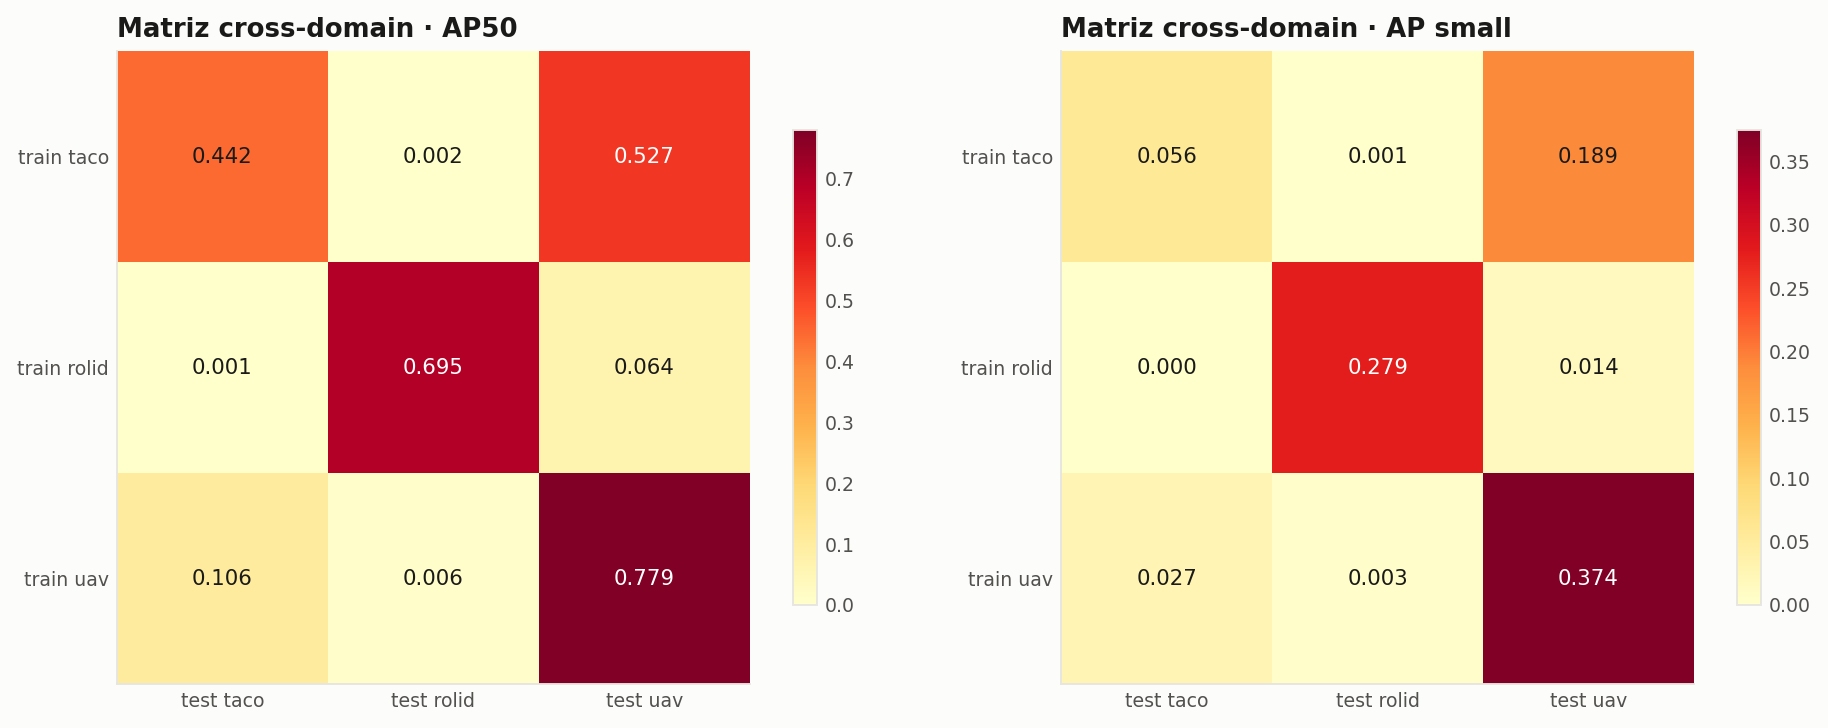
\includegraphics[width=0.80\linewidth]{matriz_cross_domain_final.png}
\end{center}
Media in-domain de 0.639 AP$_{50}$; cruzada, 0.118. El dominio dashcam es una
\textbf{isla} (AP$_{50}\le 0.064$ en ambas direcciones): su objeto mediano de
22 px cae bajo el ancla FPN m\'inima de 32 px. Mano$\rightarrow$dron retiene
el 68\% --- la escala, no la apariencia, domina la brecha.
}

\column{0.5}
\block{La higiene del split cambia conclusiones}{
\begin{center}
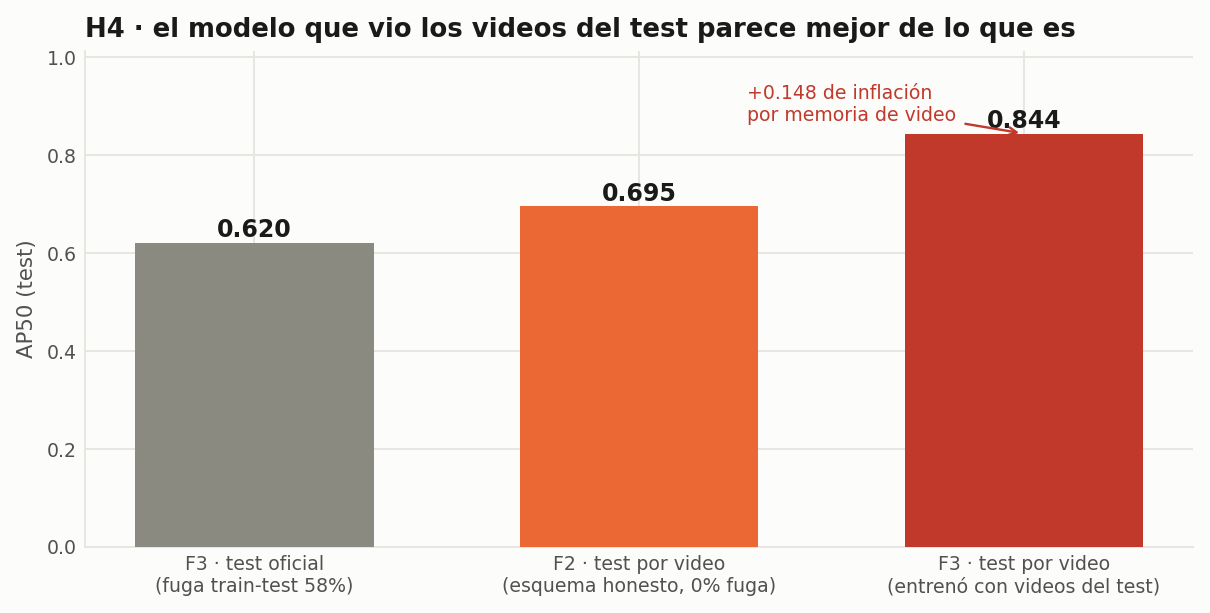
\includegraphics[width=0.58\linewidth]{fuga_oficial_vs_video.png}
\end{center}
Sobre el \emph{mismo} test limpio, el modelo entrenado con el split oficial
fugado marca \textbf{0.844 contra 0.695} del entrenado limpio: \textbf{+21\%
relativo} --- escenas memorizadas, no generalizaci\'on. El split por video lo
elimina a costo cero.
}
\end{columns}

% ═════════════════════ ROW 4 ═════════════════════
\begin{columns}
\column{0.5}
\block{Palancas baratas: la resoluci\'on}{
\begin{center}
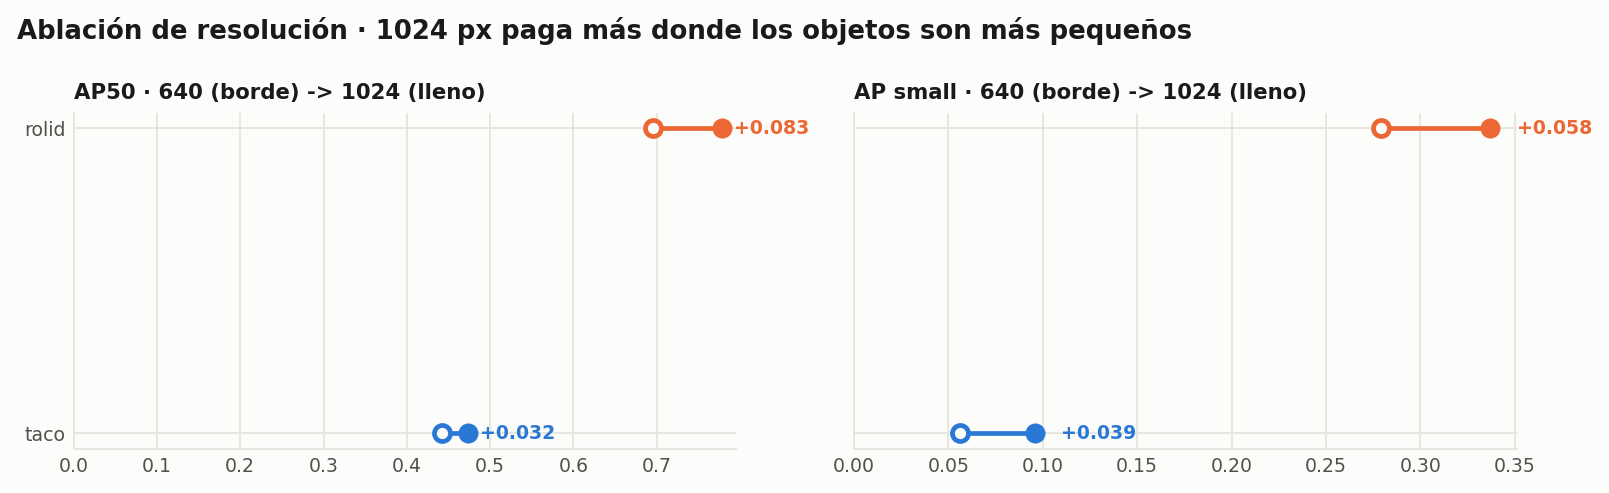
\includegraphics[width=0.85\linewidth]{ablacion_resolucion.png}
\end{center}
Las ganancias se concentran donde los objetos son m\'as peque\~nos: dashcam
+8.3 AP$_{50}$ / +5.8 AP$_S$; mano +3.2 / +3.9. Granularidad: excluir el vidrio
marginal (38 instancias de test, AP$_{50}$ 0.049) sube las cinco clases
restantes +0.014 AP$_{50}$ en promedio.
}

\column{0.5}
\block{41M contra 2.6M de par\'ametros, mismos splits}{
\begin{center}
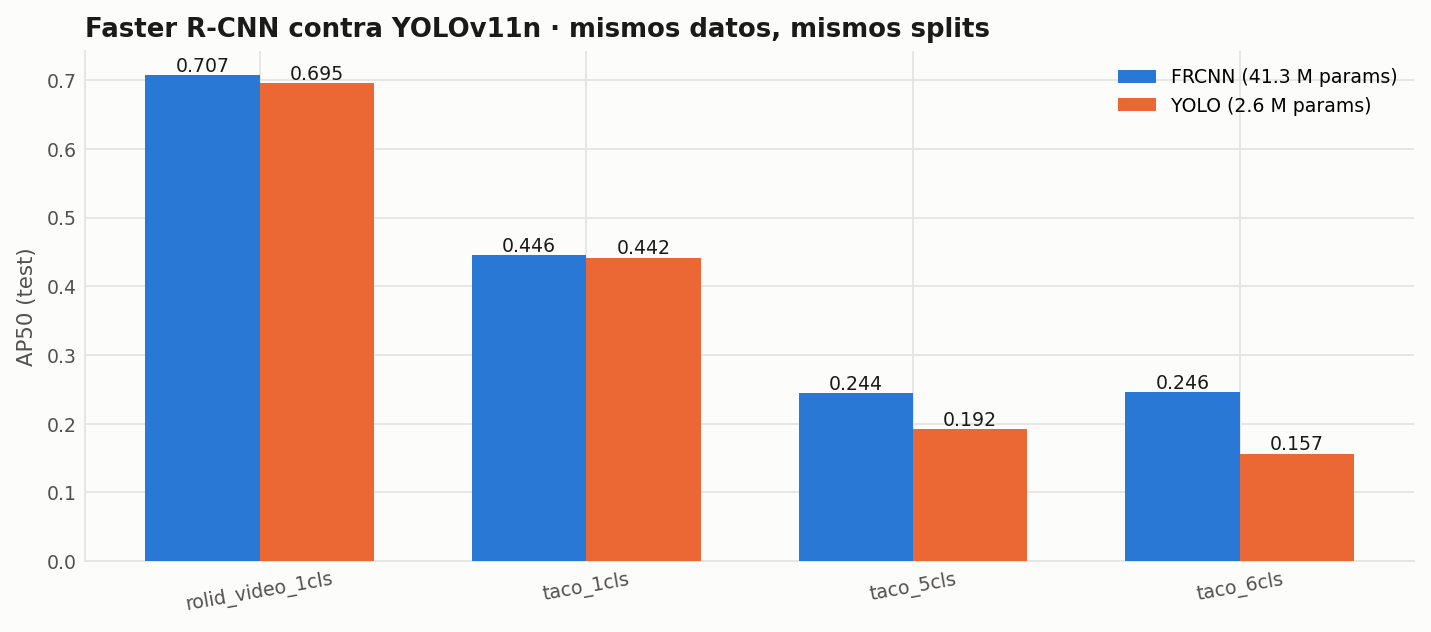
\includegraphics[width=0.70\linewidth]{comparativa_familias.png}
\end{center}
YOLOv11n queda a 1--4 puntos de AP$_{50}$ de Faster R-CNN en basura de una
clase (0.695 contra 0.707 en dashcam) --- el despliegue ligero es viable. La
brecha se abre en materiales (0.157--0.192 contra 0.244--0.246). FCN: 0.577 de
IoU; recortes VGG-16: 97.8\% de exactitud con evidencia CAM sobre el objeto.
}
\end{columns}

% ═════════════════════ ROW 5 ═════════════════════
\begin{columns}
\column{0.58}
\block{Por qu\'e fallan: anatom\'ia del error con TIDE}{
\begin{center}
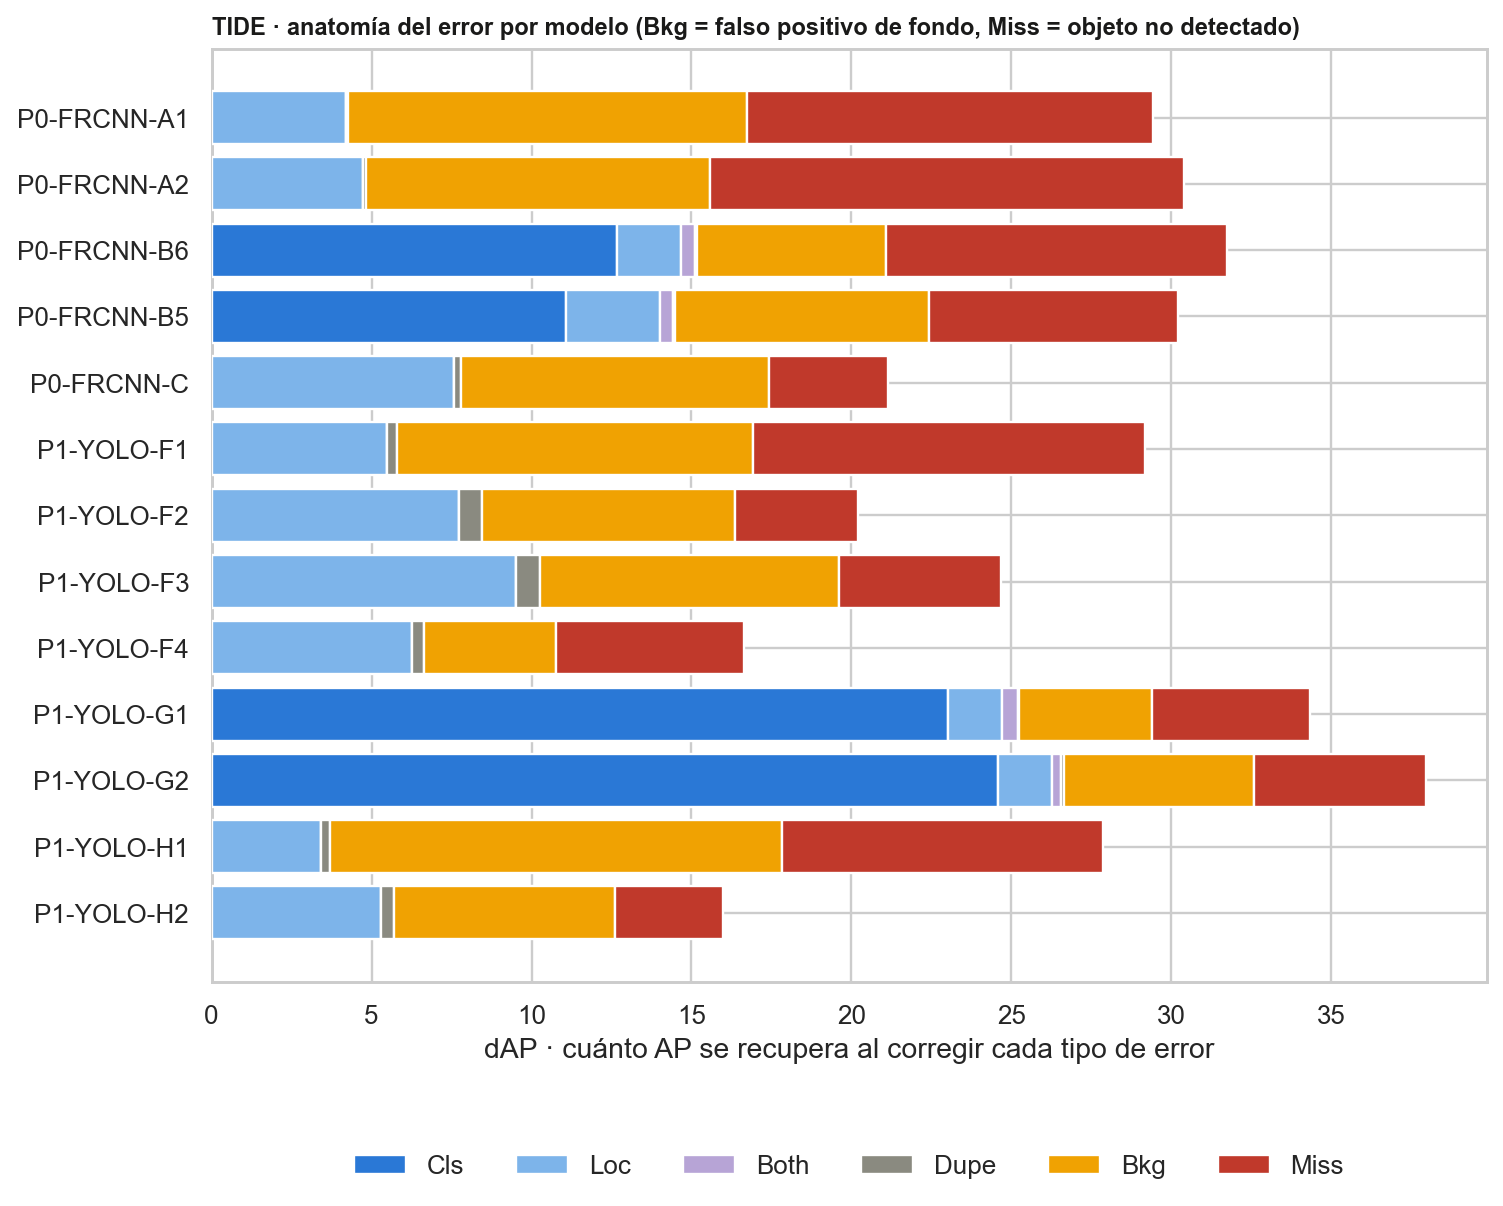
\includegraphics[width=0.42\linewidth]{tide_descomposicion.png}
\end{center}
Los multiclase pierden hasta \textbf{24.6 dAP por clasificaci\'on} contra 1.7
por localizaci\'on: el cuello de botella es nombrar el material, no encontrar
la basura; los dashcam in-domain casi no fallan por Miss.
}

\column{0.42}
\block{Conclusiones y reproducibilidad}{
\begin{itemize}
\item \textbf{A\'un no hay modelo universal de basura}: el ajuste por dominio
  (o al menos adaptar la resoluci\'on) sigue siendo obligatorio con sensores
  mixtos.
\item \textbf{Auditar antes de entrenar}: una fuga escondida reescribe un
  benchmark; los datasets con estructura de video deber\'ian publicar
  identificadores de grupo.
\item \textbf{Detectar agn\'ostico a la clase y clasificar recortes}: TIDE
  aboga por desacoplar el material (97.8\% en recortes) de la detecci\'on.
\end{itemize}
\vspace{3mm}
\textbf{Tres rutas publicadas:} demo con pesos preentrenados sobre cualquier
foto ($\sim$5 min, CPU) \,·\, regenerar cada n\'umero del paper desde los
artefactos ($\sim$10 min) \,·\, pipeline completo desde datos p\'ublicos.
C\'odigo, pesos, splits y video: \textbf{github.com --- se publica con la
entrega del curso.}
}
\end{columns}

\end{document}
